\documentclass[oneside]{amsbook}
\usepackage{amsmath}
\usepackage{amsthm}
\usepackage{amssymb}
\usepackage{mathtools}
\usepackage{hyperref}
\usepackage{cleveref}
\usepackage{enumerate}
\usepackage{subcaption}
\usepackage{comment}
\usepackage{parskip}
\usepackage{xcolor}
\usepackage{tikz-cd}
\usepackage{tcolorbox}
\newtheorem{theorem}{Theorem}
\newtheorem{lemma}{Lemma}
\newtheorem{remark}{Remark}
\newtheorem{definition}{Definition}
\renewcommand*{\d}{\mathrm{d}}

\begin{document}
\tableofcontents
\section*{Abstract}
Contact geometry is the study of odd-dimensional smooth manifolds with so called contact structures, specific hyperplane distributions $\xi = \ker \alpha$ that have to satisfy a certain relation, the contact condition
\[
    \alpha \wedge (\d \alpha)^n \neq 0.
\]
A manifold can have multiple different contact structures, which can be either rigid (in which case one speaks of a "tight" manifold) or flexible (in the sense that they satisfy an h-principle). Such contact manifolds are then called overtwisted.
To illustrate this dichotomy, consider the sphere $S^3$. It has precisely one tight contact structure, but infinitely many overtwisted contact structures, corresponding to the infinitely many homotopy classes of 2-plane fields on the 3-sphere. There are other examples where there are infinitely many or no tight contact structures on a contact manifold.
A further interesting property of contact manifolds comes from the fact that contact geometry is the odd-dimensional counterpart to symplectic geometry: Often, it is possible to view a contact manifold as the boundary of a symplectic manifold. Manifolds that are in this sense "fillable" are always tight. The contrary, however, doesn't need to hold and one can ask the question under which conditions such tight, but non-fillable manifolds exist.
Bowden, Gironella, Moreno and Zhou have shown in a recent paper that there exist homotopically standard, non-fillable but tight contact structures on all spheres $S^{2n+1}$ with $n >= 2$.

Starting with a specific open book decomposition of $S^{2n-1}$, one can construct a contact form on this manifold using a well-known construction by Thurston-Winkelnkemper. Then, according to Bourgeois, this contact structure can be extended to a tight contact structure on $S^{2n-1}\times T^2$.
Applying subcritical surgery (preserving the tightness), one can kill the topology of the $T^2$-factor and obtain a tight contact structure on $S^{2n+1}$. Because of the special way of constructing it, one can show that it is non-fillable, but still homotopically standard.
\chapter{Introduction}
As mentioned in the abstract, the dichotomy between tight and overtwisted is a fundamental concept in contact geometry.
First insights about these attributes were gained when, early in the development of the field, 
Eliashberg discovered the ``overtwisted disk".
If a threedimensional contact manifold admits an embedding of such a special disk, it is called overtwisted.
As mentioned in the abstract, such contact structures satisfy an $h$-principle.
An $h$-principle holds whenever a class of geometric structures is classified, 
up to homotopy, by its underlying topological structures (see \cref{sec:h_principle}).
In this case, the more general set are almost contact structures, where an almost contact structure
is simply the underlying topological structure of a contact structure.
Any such almost contact structure is homotopic to an overtwisted contact structure.
This is why overtwisted contact structures are comparably uninteresting: They exist
in abundance and can be classified by purely topological methods.

Tightness, another property of contact structures, was soon proved to be equivalent to ``not overtwisted".
Tight contact structures, however, are far more difficult to classify or even find than overtwisted ones.
Understanding tightness has since been a big motivating question in contact geometry.

The first systematic step in the direction of understanding tightness was the seminal work
by Eliashberg--Gromov \cite{Gromov85, Eliashberg91}. Using holomorphic curves, they proved that any type of fillability implies tightness.
Before moving on to the explanation of fillability, it is worth saying a few words on holomorphic curves.
Gromovs idea to use that technique for the proof was really visionary. 
Until today, all approaches for proving tightness are based on holomorphic curves 
The rough idea of Gromov--Eliashberg was to assume that there is a holomorphic disk, 
and then find a contradiction by constructing a suitable moduli space of holomorphic disks.
Nowadays, tools like contact homology (or similar homology theories) are all based on holomorphic curves, too.
In fact, it is an open question whether tightness can be understood fully on the basis of holomorphic curves 
or if other tools will be necessary in some cases to detect tightness.

Fillability is another important aspect of contact geometry, based on its relation to symplectic geometry.
While contact manifolds are always odd-dimensional, symplectic geometry is the corresponding concept in even dimensions.
Manifolds that are equipped with a closed nondegenerate 2-form are called symplectic. They are related
to contact manifolds in many ways.
For example, a hypersurface in a contact manifold with a transversal contact vector field
induces a convex splitting of this hypersurface: There is the so-called dividing set (a contact submanifold)
which divides the hypersurface into Liouville domains, i.e. exact symplectic manifolds (cf. \cref{sec:convex_decomposition}).

The main connection between symplectic and contact manifolds, however, is the concept of fillability:
A contact manifold is (strongly) fillable if it is the smooth boundary of a symplectic manifold and
near the boundary, the symplectic form $\omega$ is equal to $\d \alpha$.
For example, the standard contact structure on the sphere $(S^3, \xi)$ is fillable
by the standard symplectic structure on the ball $(B^4, \omega)$.

Now, as the word ``strongly" already suggests, there are several variants of fillability:
A contact manifold can be (Wein-)Stein fillable, Liouville fillable, (strongly) fillable or weakly fillable.
From left to right, there are less and less conditions to be satisfied, i.e. there is a sequence
of implications from the left to the right. 
Eliashberg--Gromovs result adds tightness to the right end of these implications.

In other words, there is a chain of inclusions from 
Weinstein- and Liouville- over strongly and weakly fillable to tight contact manifolds.
In three dimensions, these inclusions were all proven to be strict, see \cref{fig:fillability}.
\begin{figure}
    \begin{align*}
        \{\text{Weinstein fillable}\} \stackrel{\text{\cite{Bowden12}, \cite{BCS14}}}{\subsetneq} 
        \{\text{Liouville fillable}\} \stackrel{\text{\cite{Ghiggini05}, \cite{Zhou21}}}{\subsetneq}\\
        \{\text{Strongly  fillable}\} \stackrel{\text{\cite{Eliashberg96}, \cite{BGM22}}}{\subsetneq}
        \{\text{Weakly    fillable}\} \stackrel{\text{\cite{EH02}, \cite{MNW13}}}{\subsetneq}
        \{\text{Tight}\}
    \end{align*}
    \caption{Hierarchy of fillability in three dimensions (first citation) and in higher dimensions (second citation)}
    \label{fig:fillability}
\end{figure}

Basically all of the concepts explained before have been generalized to higher dimensions.
One example where this was not straightforward is the generalization of overtwistedness: 
After a long process, multiple potential definitions were shown to be equivalent in arbitrary dimensions in \cite{BEM15}.

Another example is that there is a similar hierarchy of fillabilities in higher dimensions. 
Most definitions generalize to higher dimensions in a straightforward way. Tightness can just be defined as \textit{not overtwisted}.
It turns out that the same chain of inclusions is true in higher dimensions, too.
Proving the strictness of these inclusions took another few years, but now all inclusions are known to be strict also in higher dimensions, 
see \cref{fig:fillability}.

Often, however, these proofs of strictness simply construct very specific counterexamples with a very specific underlying smooth manifold.
This leads to the question whether the strictness of these inclusions is due to specific geometric properties of the counterexamples.
Bowden--Gironella--Moreno--Zhou \cite{BGMZ22} provide a negative answer to this question by showing that tight but
non-fillable contact structures exist in every almost contact class that admits a tight structure (in $\dim = 5$, there is an additional assumption, namely $c_1\neq 0$).
This proves that there really is a inherently contact geometric difference between tightness and fillability
that can't be attributed to specific properties of the underlying smooth topology.

The proof starts with first establishing a more specific theorem: There are homotopically standard, tight, but non-fillable contact structures on the sphere.
Then, by so called ``contact connected sum" (a connected sum operation that respects the contact structure),
the general result follows.

Also, they prove that any sphere in $\dim \geq 7$ admits homotopically standard Liouville- but not Weinstein-fillable contact structures
and, analogously, deduce a more general statement from this via contact connected sum.
As weak and strong fillability are equivalent on the sphere, there are two remaining questions along this line of research:
\begin{itemize}
    \item Is there a Liouville- but not Weinstein-fillable contact structure on $S^5$?
    \item Does a higherdimensional sphere admit strongly, but not Liouville-fillable contact structures?
\end{itemize}

This thesis focuses on the first theorem of \cite{BGMZ22}: $S^{2n+1}$ admits a homotopically standard, tight, but non-fillable contact structure
for any $n \geq 2$. In fact, as the case for $n = 2$ is similar, but technically more difficult, it is omitted.

The chapters of this thesis correspond to the three main steps of the proof. First, one constructs a homotopically standard contact structure on $S^{2n+1}$.
This contact structure is then, secondly, shown to be tight.
Thirdly, non-fillability is deduced.

The starting point of \cref{chap:construction} is the famous Giroux-correspondence.
Giroux disvovered that contact structures are closely related with open book decomposition.
An open book decomposition really is a very intuitive concept: In a manifold $M^n$, find a codimension two submanifold $B^{n-2}$
s.t. there is a fibration $p\colon M\setminus B \to S^1$. $B$ is then called ``binding" and the fibers $p^{-1}(\theta)$ are the pages of the open book 
(see \cref{fig:open_book}).

\begin{figure}
    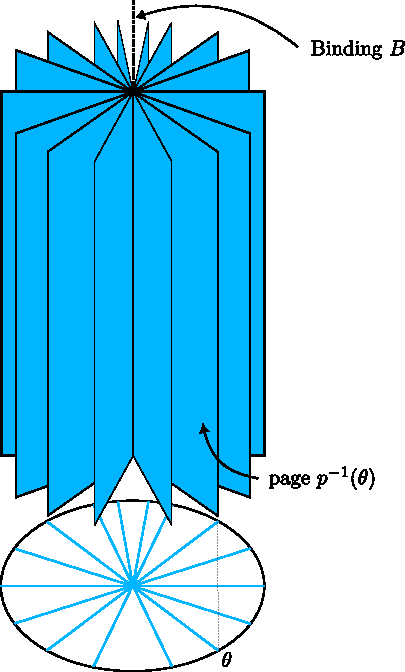
\includegraphics{images/open_book.pdf}
    \caption{Open Book Decomposition}
    \label{fig:open_book}
\end{figure}

The Giroux correspondence states that in 3 dimensions, there is a bijection (modulo technical details) between contact structures
and open book decompositions.
In higher dimensions, similar statements hold, in particular any open book decomposition leads to a corresponding supported
contact structure via the Thurston-Winkelnkemper-construction.
This is used in the proof in order to construct a contact structure that is different from the standard contact structure on $S^{2n+1}$.

Constructing a tight contact structure is not so easy: The standard way would be to take the boundary of some symplectic manifold,
but then it is of course fillable, so this approach can't be used here.
Even though there are many procedures that make a contact structure overtwisted (e.g. adding a Lutz twist), tightening procedures are very rare.
Only the Bourgeois construction was known to often yield tight contact structures. 
A recent preprint by Avdek and Zhou now proves that, in fact, Bourgeois manifolds are always tight \cite{AZ24}.
Therefore, the next step in the proof is to apply the Bourgeois construction, resulting in a Bourgeois manifold $S^{2n-1} \times T^2$.
Clearly, this has the wrong topology, so the final step in the construction is to kill the $T^2$-factor with
subcricital contact surgeries, establishing a homotopically standard contact structure on the sphere $(S^{2n+1},\xi_\text{new})$.

In \cref{chap:tightness}, one uses Reeb dynamics and holomorphic curves hidden in the framework of contact homology to prove that $\xi_\text{new}$
is really tight.

Finally, \cref{chap:nonfillable} finds a contradiction if the manifold was fillable. So first, assume it is fillable.
The largest part then is devoted to proving that fillability implies a certain property for specific homology classes
(the homological obstruction theorem).
As the theorem is easier to prove for $S^{2n-1} \times T^2$ instead of the surgered manifold $S^{2n+1}$,
this thesis covers only the proof for the homological obstruction theorem for $S^{2n-1} \times T^2$ according to \cite{BGM22}. 
The proof in the general case is similar.
Then, in the final section, a homology class as described in the homological obstruction theorem is constructed.
However, it doesn't satisfy the required property, thus establishing the desired contradiction.

\chapter[Construction]{The Construction: A homotopically standard contact structure on the Sphere}\label{chap:construction}
\section{Outline}
The goal is to find homotopically standard, tight, non-fillable contact structures on the sphere $S^{2n+1}$ for $n \geq 2$.
In this work, only the easier case $n \geq 3$ will be covered.
As $(S^{2n+1}, \xi_\mathrm{std})$ is defined as the contact boundary of the standard symplectic ball $(D^{2n+2}, \omega_\mathrm{std})$,
it is fillable by definition.
Hence, one needs a different contact structure.
This chapter explains how to construct a homotopically standard contact structure on the sphere in a way that at first might not seem very intuitive,
hoping that in the end it will be different from $\xi_\mathrm{std}$.
Later, in \cref{chap:tightness} and \cref{chap:nonfillable}, it will be shown that, as desired, this contact structure really is tight and non-fillable 
(and hence different from $\xi_\mathrm{std}$).
The starting point for the whole construction is a Milnor open book, i.e. a certain kind of decomposition of $S^{2n-1}$ that comes from
Milnors work on hypersurface singularities \cite{Milnor69}.
By the Giroux correspondence, there is a contact structure on this manifold.
In this case, part of the Giroux correspondence can be realized by an explicit construction due to Thurston-Winkelnkemper.
Now, a construction due to Bourgeois (\cite{Bourgeois02}) extends the resulting contact structure on $S^{2n-1}$ to $S^{2n-1}\times T^2$.
By applying smooth surgery, one can kill the homology in the $T^2$-factor and so obtain $S^{2n+1}$.
By an $h$-principle due to Eliashberg--Murphy (\cite[section 12.4]{EM02}), the surgeries can be realized as contact surgeries.
This completes the construction as now one has a contact structure on $S^{2n+1}$.
Finally in \cref{homotopically_standard}, it will be explained why the contact structure is homotopically standard.
\section[The Milnor open book]{Raw material for the construction: The Milnor open book} \label{sec:milnor}
Define $f\colon \mathbb C^n \to \mathbb C$ by
\[
    (z_0, \dots, z_{n-1}) \mapsto z_0^k + z_1^2 + \dots z_{n-1}^2.  
\]
Consider the sphere $S^{2n-1} \subset \mathbb C^n$.
The intersection $f^{-1}(0) \cap S^{2n-1}$ is the so called Brieskorn sphere $B = \Sigma_{n-1}(k,2,\dots,2)$.
On the complement $S^{2n-1} \setminus B$, the map
\[
    \pi_f\colon S^{2n-1}\setminus B \to S^1\colon (z_0, \dots, z_{n-1}) \mapsto \frac{f(z_0, \dots, z_{n-1})}{|f(z_0, \dots, z_{n-1})|}
\]
is a fibration over $S^1$, the Milnor fibration.
According to \cite[Lemma 6.1]{Milnor69}, the fibers are smooth $2n-2$-dimensional manifolds with boundary $B$.
It is well-known that such a fibration is precisely an open book decomposition (of $S^{2n-1}$).

If the dimension is high enough, the Brieskorn sphere is not just connected, but actually a topological sphere.

According to \cite[Thm 6.5]{Milnor69}, the pages of this open book (i.e. the Milnor fibers) have the homotopy type of a bouquet of spheres 
$S^{n-1} \vee \dots \vee S^{n-1}$.
It follows from the Hurewicz theorem that 
\[
    H_0 = \mathbb Z, \qquad H_i = 0, \; 0 < i < n \qquad \text{and } H_n = \pi_n.
\]
\cite[Theorem 9.1]{Milnor69} implies that $H_n = \pi_n = \mathbb Z^{k-1}$.

%Mention the properties that Agustin told me
%- looks like spheres merged at one point
%- homotopy of half-dimension CW complex
%- homology properties?
% -> for all of this see Milnor hypersurface singularities
\section[The Thurston-Winkelnkemper-construction]{From open books to contact structures: The Thurston-Winkelnkemper construction}
An open book in itself is of no use to the proof - a contact structure is needed! 
This section makes a special case of one direction of the Giroux correspondence explicit 
by providing a construction that takes an open book as input
and returns a contact structure as output.

Later, it will be important that the resulting contact structure is supported by the open book decomposition.
\begin{definition}\label{def:support}
    Let $(B,p)$ be an oriented open book decomposition of the oriented manifold $M$.
    A contact structure $\xi = \ker \alpha$ on $M$ is said to be \textbf{supported} by the open book decomposition $(B,p)$ of $M$ if
    \begin{enumerate}[(i)]
        \item the contact form $\alpha$ induces the positive orientation of $M$ ($\alpha \wedge (\d \alpha)^n > 0$)
        \item the 2-form $\d \alpha$ induces a symplectic form on the interior of each page, defining its positive orientation
        \item the 1-form $\alpha$ induces a positive contact form on $B$, i.e. 
        \[ 
            \alpha|_{TB} \wedge (\d \alpha|_{TB})^{(n-2)} > 0.
        \]
    \end{enumerate}
\end{definition}



\subsection*{Abstract open books}
Instead of defining an open book via a map that induces binding and pages, one can also define it by starting from the page and defining
a ``monodromy" map, i.e. a map that determines how the page changes if one follows the page $360^\circ$ around the binding.
This is based on the concept of a mapping torus.

\begin{definition}[mapping torus]
    Let $\Sigma$ be a smooth manifold with boundary $\partial \Sigma$
    and $\phi: \Sigma \to \Sigma$ a diffeomorphism that is equal to the identity close to $\partial \Sigma$.
    The mapping torus $\Sigma(\phi)$ is given by
     $[0,2\pi] \times \Sigma/\sim$ where
     \[
        (2\pi, x) \sim (0, \phi(x)). 
     \]
     The generalized mapping torus requires as additional data a smooth function $\overline{\varphi}: \Sigma \to \mathbb R^+$ that is constant near $\partial \Sigma$. Then,
     \[
        \Sigma_{\overline{\varphi}}(\phi) \coloneqq \mathbb R \times \Sigma/\sim \quad \text{where} \quad  (\theta, x) \sim (\theta - \overline{\varphi}(x), \phi(x)).
     \]
\end{definition}

Starting with a mapping torus $\Sigma(\phi)$, one can construct an abstract open book $M(\phi)$ with binding $\partial \Sigma$ (see \cref{fig:open_book}),
where the page $\overline{p^{-1}(\theta)} = \Sigma$ and $B = \partial \Sigma$.
Define
\[
    M(\phi) \coloneqq \left(\Sigma(\phi) \cup D^2 \times \partial \Sigma\right)/\sim
\]
and identify
\[
    [x \in \partial \Sigma, \theta] \sim (r=1, \varphi = \theta, x).
\]


\subsection*{The construction}

Let $\Sigma^{2n}$ be a Liouville domain. 
In particular, it is a compact manifold admitting an exact symplectic form $\omega = \d \beta$ 
s.t. on the boundary $\partial \Sigma$, a contact form $\beta_\partial$ is induced.
Let the boundary be connected (i.e. the binding is also connected).
Let the monodromy map $\phi$ be an exact symplectomorphism of $(\Sigma, \omega)$,
equal to the identity near the boundary $\partial \Sigma$ 
(exactness is not necessary according to \cite{Geiges08}, as it can be obtained via a suitable isotopy of the symplectomorphism).
An exact symplectomorphism $\phi$ of $(\Sigma, \omega)$ is such that
\[
    \phi^*(\beta) - \beta \eqqcolon \d \overline{\varphi}  
\]
is exact, i.e. there exists such a function $\overline{\varphi}$ on $\Sigma$ (of course only defined up to adding a locally constant function. Choose it in such a way that it only takes positive values).
The 1-form 
\[
    \alpha \coloneqq \beta + \d \varphi
\]
is a contact form on $\mathbb R \times \Sigma$:
\[
    \alpha \wedge (\d \alpha)^{n} = (\beta + \d \varphi)\wedge \underbrace{(\d \beta)^n}_{\eqqcolon \Omega} = \beta \wedge \Omega + \d \varphi \wedge \Omega = \d \varphi \wedge \Omega,
\]
where $\Omega$ is a volume form on $\Sigma$ (as $\beta$ is a symplectic form).
The term $\beta \wedge \Omega$ vanishes because both are forms on $\Sigma$, but $\Omega$ is already a top-level form.
The resulting form is a wedge product of two volume forms on the product manifolds and therefore a volume form on $\mathbb R \times \Sigma$.

Now consider the transformation that induces the generalized mapping torus
\[
    F \coloneqq (\varphi, x) \mapsto (\varphi - \overline{\varphi}(x), \phi(x)).    
\]
Remember that $\varphi$ only takes positive values, i.e. the mapping torus is well-defined.
The 1-form $\alpha$ is invariant under this transformation:
\begin{align*}
    F^*(\alpha) &= F^*(\beta) + F^*(\d \varphi)&&|\;\beta\text{ is independent of }\varphi\\
    &= \phi^*(\beta) + \d F(\varphi)&&|\text{ definition of }\overline{\varphi}, F\\
    &= \beta + \d\overline{\varphi} + \d \varphi - \d \overline{\varphi}\\
    &= \alpha.
\end{align*}
It follows that $\alpha$ descends to a contact form on $\Sigma_{\overline{\varphi}}(\phi)$. 

In the following, it will be necessary to have an adapted gluing construction for the abstract open book coming from a generalized mapping torus.
The page $\Sigma$ is Liouville, i.e. there exists a Liouville vector field $X$ which is transversal to the boundary $\partial \Sigma$.
This vector field induces a coordinate $s$ on a collar neighborhood of the boundary $[-1,0] \times \partial \Sigma$.
Then, the symplectic form is given by $\d \left(e^s\beta_\partial\right)$ where $s$ is the collar parameter, i.e. $X = \partial s$.

Close to $\partial \Sigma$, $\phi$ is equal to the identity and therefore $\d \overline{\varphi}$ is locally constant (hence constant, as $\partial \Sigma$ is connected).
If necessary, reparametrize the neighborhood so that $\overline{\varphi}$ is constant on $[-1,0]\times \partial \Sigma$.

Now, take a look at
\[
    M \coloneqq \left(\Sigma_{\overline{\varphi}}(\phi)\; \dot\cup\; \left(D_2^2 \times \partial \Sigma\right)\right)/\sim.
\]
\begin{figure}
    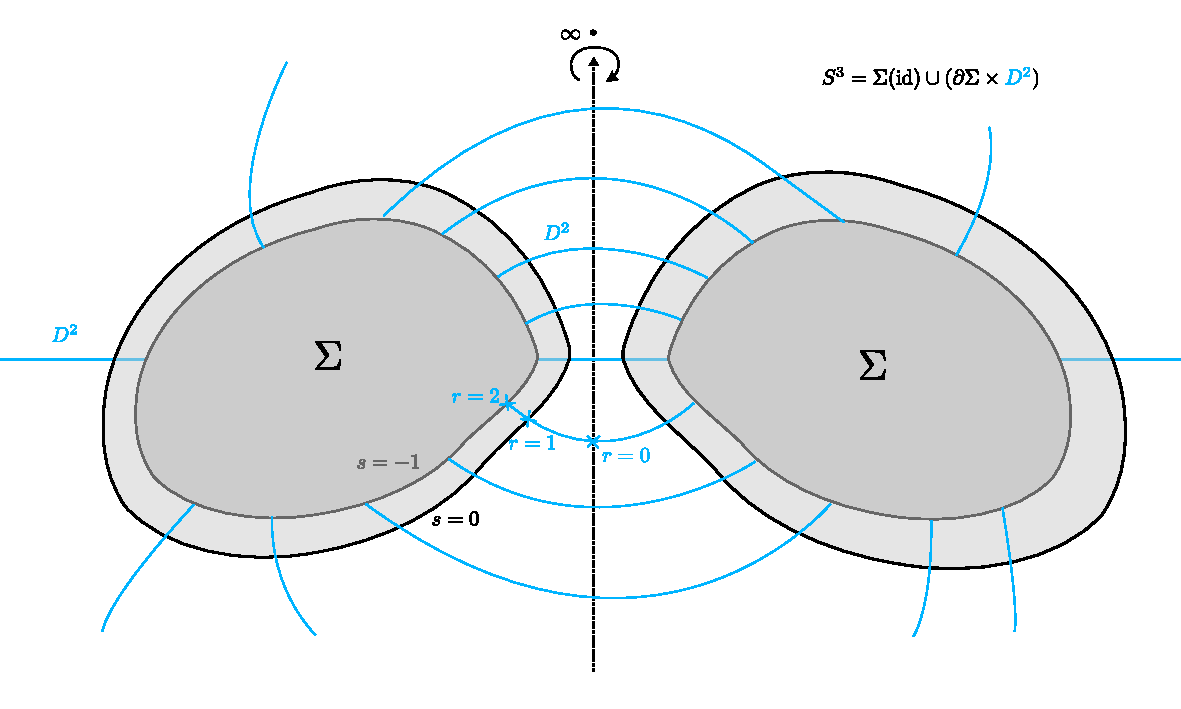
\includegraphics[width=\textwidth]{../images/abstract_open_book_gluing.pdf}
    \caption[Gluing an abstract open book]{Detailed gluing process of a generalized abstract open book decomposition for $S^3$}
    \label{fig:abstract_open_book_gluing}
\end{figure}

A simple linear reparametrization will make the notation a lot easier: As $\overline{\varphi}$ is constant on the neighborhood under consideration, just pretend that $\overline{\varphi} = 2\pi$.
Then identify 
\[
    (s, x, \varphi) \in [-1,0] \times \partial \Sigma \times S^1 \subset \Sigma_{\overline{\varphi}}(\phi)
\]
with
\[
    (x, s = 1-r, \varphi) \in \partial \Sigma \times D_2^2 \eqqcolon \mathcal{N}
\]
where $(r, \varphi)$ are polar coordinates on $D_2^2$, i.e. a collar neighborhood of $\Sigma$ is identified with an annulus in $D_2^2$
(See \cref{fig:abstract_open_book_gluing} for a drawing in three dimensions).

Now choose the ansatz
\[
    \alpha_\text{ext} \coloneqq h_1(r) \beta_\partial + h_2(r) \d\varphi
\]
for the extension of the contact form over $\mathcal{N}$.
On the gluing area (i.e. $1 \le r \le 2$), $\alpha_\text{ext}$ has to agree with $\alpha = \beta + \d \varphi = e^s \beta_\partial + \d \varphi$,
i.e.
\[
    h_1(r) = e^s = e^{1-r} \qquad h_2(r) = 1.
\]
In order to ensure smoothness at $r=0$, set $h_1(r) = 2 - r^2$ and $h_2(r) = r^2$ in a small neighborhood of $r = 0$. Then,
\[
    \alpha_\text{ext}|_0 = 2\beta_\partial
\]
Further,
\[
    \d \alpha_\text{ext} = h_1'(r)\d r\wedge \beta_\partial + h_1(r) \d \beta_\partial + h_2'(r) \d r \wedge \d\varphi
\]
and
\[
    (\d \alpha_\text{ext})^n = n\cdot \d r\wedge (h_1'(r) \beta_\partial + h_2'(r) \d\varphi) \cdot h_1(r)^{n-1}(\d \beta_\partial)^{n-1} + \underbrace{h_1(r)^n (\d \beta_\partial)^n}_{=0},
\]
where the second term vanishes because $(\d \beta_\partial)^n$ is a $2n$-form on $\partial \Sigma^{2n-1}$.
% the first and third term together can occur at most once in a term becuase of the dr
% as dbeta is a two-form, the order doesn't matter and it commutes with the other terms
Finally,
\begin{align*}
    \alpha_\text{ext} \wedge (\d \alpha_\text{ext})^n =& \;h_1(r)n h_1(r)^{n-1} h_2'(r) \cdot&&\beta_\partial \wedge \d r \wedge \d \varphi \wedge (\d\beta_\partial)^{n-1}\\
    &+ h_2(r)n h_1(r)^{n-1}h_1'(r) \cdot&&\d \varphi \wedge \d r \wedge \beta_\partial \wedge (\d\beta_\partial)^{n-1}\\
    =& n h_1(r)^{n-1}(h_1h_2'(r) - h_2h_1'(r)) \cdot &&\beta_\partial \wedge (\d\beta_\partial)^{n-1} \wedge \d r \wedge \d \varphi\\
    =& n h_1(r)^{n-1}\det \begin{pmatrix}
        h_1(r) & h_2(r)/r\\
        h_1'(r) & h_2'(r)/r
    \end{pmatrix} \cdot &&\beta_\partial \wedge (\d\beta_\partial)^{n-1} \wedge r \d r \wedge \d \varphi\\
\end{align*}
As $\beta_\partial$ is a contact form on $\partial \Sigma$, $\beta_\partial \wedge (\d\beta_\partial)^{n-1}$ is a positive volume form on $\partial \Sigma$. 
Furthermore, $r \d r\wedge \d \varphi$ is a positive volume form on the disk $D_2^2$. 
As a result, the right term of the result is a volume form on $\mathcal{N} = \partial \Sigma \times D_2^2$.
The left term shows that $h_1(r)$ mustn't have any zeros for $r \in [0,2]$ and that $(h_1(r), h_2(r))$ must never be parallel to $(h_1'(r), h_2'(r))$, i.e.
\[
    h_1(r)^{n-1}\det \begin{pmatrix}
        h_1(r) & h_2(r)/r\\
        h_1'(r) & h_2'(r)/r
    \end{pmatrix} > 0 \qquad \forall r \in [0,2].
\]
(Close to zero, the determinant is given by $2 \cdot 2 - 0 \cdot 0 = 4 > 0$).
Figure 4.7 in \cite{Geiges08} proves the existence of such a pair of functions $h_1$ and $h_2$.


In total, $\alpha_\text{ext}$ induces the correct orientation on the extension and,
as $M$ is connected and orientable, on all of $M$.
In particular, condition (i) of \cref{def:support} holds and $\alpha \wedge (\d \alpha)^n = \d \varphi \wedge \Omega$ is a positive volume form on the mapping torus. 

Recall that $\omega$ is the symplectic form on $\Sigma$.
As $\Omega = (\d \beta)^n = \omega^n$, it is a $2n$-form and hence $\Omega$ is a positive volume form on $\Sigma$. 
Thus, on $\Sigma$, $\d \alpha = \d \beta = \omega$ is a symplectic form that induces the positive orientation of $\Sigma$. 
On $\mathcal{N}$, it is necessary to check that the form induced by $\d \alpha_\text{ext}$ on the pages is symplectic with the right orientation.
Inside $\mathcal{N}$, a page is given by the condition $\varphi = \mathrm{const}$, i.e. $\d \varphi = 0$.
Also,
\begin{align*}
    (\d \alpha_\text{ext})^n &= n\cdot \d r\wedge (h_1'(r) \beta_\partial + h_2'(r) \d\varphi) \cdot h_1(r)^{n-1}(\d \beta_\partial)^{n-1}\\
    &= n h_1'(r)h_1(r)^{n-1} \d r \wedge \beta_\partial \wedge (\d \beta_\partial)^{n-1}
\end{align*}

A positive volume form on $\Sigma$ must be positive on $- \partial_r, \mathfrak{b}$ where $\mathfrak{b}$ is a positive basis of a point in $\partial \Sigma$.
As $\beta_\partial \wedge (\d \beta_\partial)^{n-1}$ is a positive volume form on $\partial \Sigma$, it follows
\begin{align*}
    (\d \alpha_\text{ext})^n(- \partial_r, \mathfrak{b}) &= \underbrace{n h_1(r)^{n-1}}_{\eqqcolon A > 0} \cdot h_1'(r) \d r(-\partial_r) \wedge \underbrace{\left[\beta_\partial \wedge (\d \beta_\partial)^{n-1}\right](\mathfrak{b})}_{\eqqcolon B > 0}\\
    &= AB \cdot h_1'(r) \cdot -1\\
    &> 0,
\end{align*}
where in the last line $h_1'(r) = \frac{\d}{\d r}(2 - r^2) = -2r < 0$.
This verifies condition (ii) inside $\mathcal{N}$ and outside $\mathcal{N}$, on $\Sigma$. As a result, is must hold on the whole page.
Condition (iii) follows from the fact that on $B$, $\alpha_\text{ext} = 2 \beta_\partial$ which is a positive contact form on $\partial \Sigma$ and therefore also on $B$.

This concludes the construction of a contact structure supported by a starting open book.
As this construction will be applied to the Milnor open book, one must check that it satisfies all requirements for the construction.
Every open book is an abstract open book. For the Milnor open book, the pages are Weinstein and in particular Liouville.
The binding is connected for $\dim B \geq 3$, i.e. as soon as the open book composition has $\dim \geq 5$.
As this thesis only considers the case with $\dim S^{2n+1} \geq 7$ and the Bourgeois construction will add 2 dimensions, this suffices
in all cases that are considered here. 
The monodromy is the identity close to the binding (see e.g. \cite[section 4.2]{KvK16}).
\section[The Bourgeois construction]{From \texorpdfstring{$M$}{M} to \texorpdfstring{$M \times T^2$}{M x T2}: The Bourgeois construction}
It is not very hard to construct a contact structure on the three-torus. 
When Lutz \cite{Lutz79} discovered a contact structure on $T^5$, however,
it was natural to wonder whether there exists a contact structure on $T^{2n+1}$ for all $n \in \mathbb N$.
In order to answer this long-standing question, Bourgeois \cite{Bourgeois02} came up with a construction that takes as input a contact structure on $M$ 
and as output returns a contact structure on $M\times T^2$.
To be more precise, it requires a contact structure that is supported by an open book decomposition as an input.
However, a result by Giroux and Mohsen \cite[Theorem 7.3.5]{Geiges08} shows that to every contact structure one can find such an open book decomposition,
so that is not an obstruction, but rather part of the construction data.

\subsection{General construction}
Let $\operatorname{dim} M \geq 3$ and $(B, \pi)$ an open book decomposition of $M$ supporting $(M, \xi = \ker \alpha)$.
By definition of an open book, there is a trivial tubular neighborhood $B \times D^2$ around $B$ and there exist a radial coordinate $r$ with $r = 0$ precisely on $B$
s.t. $(r, \pi)$ form polar coordinates on this neighborhood.
Choose a smooth function $\rho$ of $r$ s.t. $\rho = r$ close to $r = 0$, $\rho'(r) > 0$ and $\rho = 1$ at $\partial D$.
Extend this function to $M$ by setting $\rho = 1$ on $M \setminus B \times D$ (see \cref{fig:rho}).
\begin{figure}
    \includegraphics*[width=\textwidth]{../images/rho.pdf}
    \caption{One-dimensional sketch of $\rho$}
    \label{fig:rho}
\end{figure}
As $\pi$ and $\rho$ are smooth functions on $M$, one can define the smooth functions $x_1 \coloneqq \rho \cos \pi$ and $x_2 \coloneqq \rho \sin \pi$ on all of $M$. 
On $B \times D^2$, they coincide with the Cartesian coordinate functions near $B$.
As always with corresponding polar- and cartesian coordinates, they satisfy
\begin{align*}
    x_1 \d x_2 - x_2 \d x_1 &= \rho^2 \cos^2 \pi \d \pi + \rho \cos \pi \sin \pi \d \rho + \rho^2 \sin^2 \pi \d \pi - \rho \cos \pi \sin \pi \d \rho\\
    &= \rho^2 (\cos^2 \pi + \sin^2 \pi) \d \pi\\
    &= \rho^2 \d \pi
\end{align*}
and, analogously,
\begin{align*}
    \d x_1 \wedge \d x_2 = \rho \d \rho \wedge \d \pi.
\end{align*}

On $M\times T^2$, choose coordinates $(\theta_1, \theta_2)$ on the torus part of the manifold.
Define
\[
    \tilde \alpha \coloneqq x_1 \d \theta_1 - x_2 \d \theta_2 + \alpha.
\]
to be a $1$-form on $M$ (where $\alpha$ is extended in the obvious way to $M\times T^2$ as the pullback $\pi_1^*\alpha$).
This is the candidate for the contact form on $M\times T^2$.
Having computed the exterior derivative and its n-th power
\begin{align*}
    \d \tilde \alpha &= \d x_1 \wedge \d \theta_1 - \d x_2 \wedge \d \theta_2 + \d \alpha,\\
    (\d \tilde \alpha)^n =& (n-1)(\d \alpha)^{n-1}\wedge (\d x_1 \wedge \d \theta_1 - \d x_2 \wedge \d \theta_2)\\
    &- n(n-1)(\d \alpha)^{n-2}\wedge \d x_1 \wedge \d \theta_1 \wedge \d x_2 \wedge \d \theta_2,
\end{align*}
one can check the contact condition:
\begin{align*}
    \tilde \alpha \wedge (\d \tilde \alpha)^n =& (x_1 \d \theta_1 - x_2 \d \theta_2 + \alpha) \wedge (n-1)(\d \alpha)^{n-1}\!\wedge (\d x_1 \wedge \d \theta_1 - \d x_2 \wedge \d \theta_2)\\
    &- (x_1 \d \theta_1 - x_2 \d \theta_2 + \alpha) \wedge n(n-1)(\d \alpha)^{n-2}\wedge \d x_1 \wedge \d \theta_1 \wedge \d x_2 \wedge \d \theta_2\\
    =& (n-1)(\d \alpha)^{n-1}\wedge(x_1\d x_2 - x_2 \d x_1)\wedge \d \theta_1 \wedge \d \theta_2\\
    &+\underbrace{\alpha\wedge(n-1)(\d \alpha)^{n-1}\!\wedge \d x_1}_{2n-\text{form on } M} \wedge \d \theta_1 - \underbrace{\alpha \wedge (n-1)(\d \alpha)^{n-1}\!\wedge\d x_2}_{2n-\text{form on } M} \wedge \d \theta_2\\
    & + n(n-1)\alpha\wedge(\d \alpha)^{n-2}\wedge \d x_1 \wedge \d \theta_1 \wedge \d x_2 \wedge \d \theta_2\\
    \intertext{$M$ has dimension $2n-1$, i.e. the middle term is 0}
    =& (n-1)(\d \alpha)^{n-1}\wedge \rho^2 \d\phi \wedge \d \theta_1 \wedge \d \theta_2\\
    & + n(n-1)\alpha \wedge (\d \alpha)^{n-2}\wedge \rho \d\rho \wedge \d \phi \wedge \d \theta_1 \wedge \d \theta_2.
\end{align*}
As this expression is a top-dimensional form, it suffices to show that its nowhere zero.
For that, one needs to employ the fact that $\alpha$ is supported by $(B, \pi)$.
By condition (ii) of \cref{def:support}, $(\d \alpha)^{n-1}$ must be a positive volume form on the pages. 
As explained in that definition, the orientation on $M$ is given by $\partial_\phi$ and the orientation of the page. 
In particular, $(\d \alpha)^{n-1} \wedge \rho \d \phi$ is a positive volume form on $M$. 
Multiplied with a second $\rho$-factor, it vanishes along $B$. 
As $\theta_1 \wedge \theta_2$ is a positive volume form on $T^2$, the first term is non-negative everywhere and positive away from 
\[
    \underbrace{B \times 0}_{\subset B \times D^2 \subset M} \times T^2.
\]
Let $\mathfrak{b}$ be a basis of the binding $B$ that is positively ordered. 
Then, $- \partial_r, \mathfrak{b}$ and thus $\mathfrak{b}, \partial_r$ are positive bases of the page (the minus disappears because the binding is odd-dimensional). 
Clearly, then, 
\[ 
    \mathfrak{a} \coloneqq \mathfrak{b}, \partial_r, \partial_\phi, \partial_{\theta_1}, \partial_{\theta_2}
\] 
is an ordered basis of $M\times T^2$.
Using $\rho'(r) \geq 0$ everywhere, it follows that $\d \rho(\partial_r)$ is non-negative.
Hence, plugging $\mathfrak{a}$ into the second term,
\begin{align*}
    &\left(n(n-1)\alpha \wedge (\d \alpha)^{n-2}\wedge \rho \d\rho \wedge \d \phi \wedge \d \theta_1 \wedge \d \theta_2\right)(\mathfrak{a})\\
    =& n(n-1) \rho \cdot (\alpha \wedge (\d \alpha)^{n-2})(\mathfrak{b}) \cdot d\rho(\partial_r) \cdot \d \phi(\partial_\phi) \cdot \d \theta_1(\partial_{\theta_1}) \cdot \d \theta_2(\partial_{\theta_2})\\
    \geq& 0.
\end{align*}
By condition (iii) of \cref{def:support}, $\alpha \wedge (\d \alpha)^{n-2}$ is positive on $B$. 
Therefore, the second term is positive on $B \times 0 \times T^2$ (hence also on a neighborhood) and non-negative everywhere else.
This proves the contact condition and $\tilde \alpha$ is indeed a contact form on $M\times T^2$.

\subsection{Example: Bourgeois and Thurston-Winkelnkemper}
Applying the Thurston--Winkelnkemper construction yields a contact form $\alpha_\text{ext}$ on
\[
    M = \left(\Sigma_{\overline{\varphi}}(\phi)\; \dot\cup\; \mathcal{N}\right)/\sim.
\]
Now, we apply the Bourgeois construction to it and obtain a contact form
\[
    \tilde \alpha_\text{ext} = \alpha_\text{ext} + x_1 \d \theta_1 - x_2 \d\theta_2
\]
on $M \times T^2$ where $\theta_1, \theta_2$ are coordinates on $T^2$
and $x_1, x_2$ are coordinates as described in the section on the Bourgeois construction, 
i.e. there is a function $\rho: M \to [0,1]$ that agrees with $r$ near the binding $B$ and we define
\[
    x_1 \coloneqq \rho \cos(p);\qquad x_2 \coloneqq \rho \sin(p).
\]

Inside $\mathcal{N}$, our projection map $p$ is given by the angular coordinate $\varphi$. Therefore,
\[
    \alpha|_\mathcal{N} = \alpha_\text{ext} = h_1(r)\beta_\partial + h_2(r)\d \varphi = h_1(r)\beta_\partial + h_2(r)\d p.
\]
In total, we obtain for the contact form on $\mathcal{U} \coloneqq \mathcal{N}\times T^2$
\[
    \tilde \alpha = h_1(r)\beta_\partial + h_2(r)\d p + \rho(r)(\cos(p) \d \theta_1 - \sin(p) \d \theta_2)
\]
Outside $\mathcal{U}$, the form is given by
\[
    \tilde \alpha = \beta + \d p + \cos(p) \d\theta_1 - \sin(p) \d \theta_2,
\]
as $\rho(r) = 1\; \forall r \geq 1$.
Collecting all the conditions on $h_1$ and $h_2$ from the last section, we require that
\begin{itemize}
    \item $h_1(r) = e^s = e^{1-r}, h_2(r) = 1$ in the gluing area ($ 1 \le r \le 2$).
    \item Smoothness around the binding and contact condition on the binding: $h_1(r) = 2 - r^2$ and $h_2(r) = r^2$ around $r = 0$.
    The $-r^2$-part is only important to have $h_1'(r) < 0$ around $0$ to satisfy the symplectic condition on the pages.
    \item Contact condition on the tubular neighborhood: \[
        h_1(r)^{n-1}\det \begin{pmatrix}
            h_1(r) & h_2(r)/r\\
            h_1'(r) & h_2'(r)/r
        \end{pmatrix} > 0 \qquad \forall r \in [0,2].
    \]
\end{itemize}

\subsection{Reeb dynamics}
We now define two functions $\mu, \nu: M \to \mathbb R$ as follows:
\[
    \mu = \begin{cases}
        \frac{\rho'}{\rho' h_1 - \rho h_1'} &\text{inside } \mathcal{U}\\
        0 &\text{outside } \mathcal{U} 
    \end{cases}  
    \quad \text{and} \quad 
    \nu = \begin{cases}
        \frac{-h_1'}{\rho' h_1 - \rho h_1'} &\text{inside } \mathcal{U}\\
        1 &\text{outside } \mathcal{U}
    \end{cases}.
\]
Both $\mu$ and $\nu$ are smooth.
First of all, we note that both are quotients of smooth functions.
We have to make sure that $\rho'h_1 \neq \rho h_1'$.
All of the involved functions are non-negative except for $h_1'$, which is constantly negative ($h_1$ needs to be chosen in such a way that $h_1'$ is nonzero). As a result,
\[
    \rho'h_1 > 0 > \rho h_1',
\]
so the denominator is always nonzero.
As $\rho$ is constantly 1 for $r \geq 1$, we see that $\mu$ is 0 for $r \geq 1$.
In particular, it is smooth everywhere. For $\nu$, setting $\rho \equiv 1$ implies $\rho' = 0$ on $r \geq 1$. Therefore, the denominator simplifies to 1 and $\nu$ is smooth, too.
\begin{lemma}
    The Reeb vector field of the contact form $\tilde \alpha$ is given by
    \[
        R = \mu(r)R_B + \nu(r)[\cos(p)\partial_{\theta_1} - \sin(p)\partial_{\theta_2}],
    \]
    where $R_B$ is the Reeb vector field of $\beta_\partial$, the contact form on $\partial \Sigma$.
\end{lemma}
\begin{proof}
    Inside $\mathcal{U}$, we compute
    \begin{align*}
        \tilde\alpha(R) &= h_1(r)\beta_\partial(R) + h_2(r)\d p(R) + \rho(r)(\cos(p) \d \theta_1 - \sin(p) \d \theta_2)(R)\\
        \intertext{$\beta_\partial$ and $\d p$ are 0 on $\partial_{\theta_i}$, $p$ and $\theta_i$ are constant on $R_B$}
        &= h_1\mu\beta_\partial(R_B) + \rho\nu(\cos(p) \d \theta_1 - \sin(p) \d \theta_2)(\cos(p)\partial_{\theta_1} - \sin(p)\partial_{\theta_2})\\
        &= h_1 \mu + \rho\nu[\cos(p)\cos(p) + \sin(p)\sin(p)]\\
        &= \frac{h_1\rho'}{\rho'h_1 - \rho h_1'} + \frac{- \rho h_1'}{\rho'h_1 - \rho h_1'}\\
        &= 1.
    \end{align*}
    Computing $\d \tilde\alpha$, we immediately drop the $\d r$-terms, as they evaluate to $0$ on $R$.
    \begin{align*}
        \d\tilde \alpha(R, \cdot) &= h_1(r)\d \beta_\partial(R, \cdot) - \rho(r)[\sin(p)\d p \wedge \d \theta_1 + \cos(p) \d p\wedge \d \theta_2](R, \cdot)
        \intertext{$\beta_\partial$ and $\d p$ are 0 on $\partial_{\theta_i}$, $\d \beta_\partial(R_B) = 0$, $p$ is 0 on $R_B$}
        &= \rho(r)\left[\sin(p)\d\theta_1(R)\d p + \cos(p)\theta_2(R)\d p\right]
        \intertext{$\d \theta_i$ is 0 on $R_B$}
        &= \rho(r)\nu(r)\left[\sin(p)\cos(p) - \cos(p)\sin(p)\right]\d p\\
        &= 0
    \end{align*}
    Outside $\mathcal{U}$, we have
    \[
        R = \cos(p)\partial_{\theta_1} - \sin(p)\partial_{\theta_2}.  
    \]
    Therefore,
    \begin{align*}
        \tilde\alpha(R) &= \beta(R) + \d p(R) + \cos(p) \d\theta_1(R) - \sin(p) \d \theta_2(R)\\
        \intertext{$\beta$ and $\d p$ are 0 on $\partial_{\theta_i}$}
        &= [\cos(p) \d \theta_1 - \sin(p) \d \theta_2](\cos(p)\partial_{\theta_1} - \sin(p)\partial_{\theta_2})\\
        &= \cos(p)\cos(p) + \sin(p)\sin(p)\\
        &= 1
    \end{align*}
    Also,
    \begin{align*}
        \d \tilde\alpha(R) &= \d \beta(R, \cdot) - \sin(p)\d p \wedge \d\theta_1(R, \cdot) - \cos(p)\d p \wedge \d \theta_2(R, \cdot)\\
        \intertext{$\beta$ and $\d p$ are 0 on $\partial_{\theta_i}$}
        &= \sin(p)\d \theta_1(R) \d p + \cos(p)\d\theta_2(R)\d p\\
        &= \sin(p)\cos(p) \d p - \cos(p)\sin(p)\d p\\
        &= 0
    \end{align*}
\end{proof}

From here on, one can compute the Conley-Zehnder-index of the periodic orbits etc. - lots of things that are blackboxed later.
Maybe state the results here for transparency.
\section{Surgery}
Carrying out the constructions of the previous sections, one starts with the Milnor open book decomposition of $S^{2n-1}$,
turns it into a contact manifold via the Thurston-Winkelnkemper construction and then constructs a
contact structure on $S^{2n-1} \times T^2$.
However, a contact structure on $S^{2n+1}$ is needed. How can this be fixed?

Surgery is, generally speaking, a procedure to change manifolds in a controlled way (see \cite{Milnor61}).
The rough idea is that the product manifold $S^p \times S^q$ can be considered either 
\begin{align}
    \text{as the boundary of } &S^p \times D^{q+1},
    \intertext{or}
    \text{as the boundary of } &D^{p+1} \times S^q.
\end{align}
Hence, given any embedding of $S^p \times D^{q+1}$ in a manifold $M$, the interior can be removed and replaced with $D^{p+1} \times S^q$.
This can be done in a smooth way (i.e. preserving the smooth structure of the manifold).

In the situation of this paper, $S^{2n-1} \times T^2$ has to be changed into $S^{2n+1}$. This can be done via surgery and the details will be explained further below.
However, preserving the smooth structure isn't enough: The contact structure has to be preserved, too.
Fortunately, there is suitable h-principle that allows to realize all the required surgeries as contact surgeries.
% Explain surgery in general and cite the relevant lemmas from mil61

\subsection{Smooth surgery}
For the details of how to realize surgery in a smooth way, consult \cite[paragraph 1]{Milnor61}.
Surgery is a quite general operation, in fact \cite[Theorem 1]{Milnor61} states that two manifolds can be transferred 
into one another by a sequence of surgeries if and only if they belong to the same cobordism class.
In particular, the Stiefel-Whitney numbers (and hence orientability) are preserved under surgery.

Let $W^n$ be a manifold, $\lambda \in \pi_p(W)$ a homotopy class and $f_0: S^p \to W \in \lambda$. When can $\lambda$ be killed?
According to \cite[Lemma 3]{Milnor61}, a homotopy group can be killed if $n \geq 2p+1$ and the induced $S^p$-bundle $f_0^*(TW)$ is trivial.
In this case, all homotopy groups $\pi_i(W)$ for $i < p$ stay unchanged, but $\pi_p(W)$ changes to $\pi_p(W)/G$ where $G$ is a subgroup containing $\lambda$.

Pick any base point $x \in M \times S^1$ and then embed $x \times S^1 \hookrightarrow M \times T^2$.
As the normal bundle to $S^1 \hookrightarrow T^2$ is trivial, it follows that also the normal bundle to $S^1 \hookrightarrow M \times T^2$ is trivial.
This yields the desired embedding and so one can kill the respective homotopy class 
(which in this case is the same as a homology class because $\pi_1 = \mathbb Z^2$ is already an abelian group).
It turns out that the second generator in $H_1$ can be killed like that, too.
$H_2$ is then isomorphic to $\pi_2$ by the Hurewicz theorem.
After proving that the respective 2-surgery is possible, one has created a manifold whose $H_1$ and $H_2$ homology groups are zero.
In fact, one can prove that all homology groups are zero after the described surgery operations.
FInally, the following two lemmata conclude the proof that the resulting manifold is diffeomorphic to a sphere.

\begin{lemma}
    A simply connected homology sphere is homeomorphic to the sphere.
\end{lemma}
\begin{proof}
    Let $M^n$ be a simply connected CW-complex that is a homology sphere, i.e. $H^0(M) = \mathbb Z$ and $H^n(M) = \mathbb Z$. 
    As $M$ is simply connected, i.e. $\pi_1(M) = 0$, the Hurewicz theorem states that
    \[
    \pi_k(M) = 0 \; \forall 1 < k < n\text{ and }\pi_n(M) = H^n(M) = \mathbb Z.
    \]
    As a result, $M$ is a homotopy sphere.
    Consider a generator $f: S^n \to M$ of $\pi_n(M)$.
    On $\pi_0$ level, it maps one connected component to one connected component, so here the induced map is obviously bijective.
    On $\pi_k$ level with $0 < k < n$, it just maps $0$ to $0$ which is an isomorphism.
    On $\pi_n$ level, one needs to show that 
    \[
        f_*: \mathbb Z = \pi_n(S^n) \to \pi_n(M) = \mathbb Z 
    \]
    is an isomorphism. The identity map is a generator for $\pi_n(S^n)$. Now $f_*(\mathrm{id}) = f$, so one obtains a generator of $\pi_n(M)$. 
    A map from $\mathbb Z \to \mathbb Z$ that sends $1$ to $1$ is a group isomorphism. These considerations show that $f$ is a weak homotopy equivalence.
    As a smooth manifold, $M$ is a CW-complex. By Whiteheads theorem it follows that $f$ is a homotopy equivalence, so the generalized Poincar\'e conjecture 
    shows that $M$ is homeomorphic to the sphere.
\end{proof}

\begin{lemma}
    A simply connected homology sphere that bounds a homology ball is diffeomorphic to the sphere.
\end{lemma}
\begin{proof}
    According to the last lemma, the homology sphere $M$ is homotopy equivalent to a sphere.

    As $W$ is a simply connected homology ball, all homotopy groups $\pi_{\ge 1}$ are 0 by the Hurewicz theorem.
    Taking any constant map on $W$ therefore is a homotopy equivalence by Whiteheads theorem, i.e. $W$ is contractible. 
    Then, cut out a ball inside $W$ and obtain a cobordism $W'$ from a sphere to $M$.
    One can prove, then, that $W'$ is an $h$-cobordism.
    Thus, by the $h$-cobordism theorem (Ranicki, Theorem 1.9), $M$ is diffeomorphic to a sphere.
\end{proof}
% Explain why all surgery can be realized in a contact way

\subsection{What is an $h$-principle?}\label{sec:h_principle}
$h$-principle stands for homotopy-principle. 
An $h$-principle holds whenever a class of geometric structures is classified, up to homotopy, by its underlying topological structures.
The term often appears in the following setting: There is an underlying set of topological objects (whatever that may be) $T$
and among them a subset $G$ of geometric (more special) objects. An $h$-principle would state that every object $x \in T$ is homotopic to an object $x \in G$.

\subsubsection*{Examples:}
\begin{itemize}
    \item A car in the plane: A car can only move in the direction of its wheels. Such paths are called holonomic. Any non-holonomic path (e.g. sliding the car
    to the right or left) can be arbitrarily close approximated by a holonomic one. In particular, it is homotopic to a holonomic path.
    The existence of an arbitrarily close approximation is often expressed by calling it a \textbf{dense} $h$-principle.
    \item Nash-Kuiper-Theorem: Any smooth embedding of $M^{n-1}$ into $\mathbb R^n$ can be arbitrarily well approximated by an isometric $C^1$-embedding. 
    In particular, any such smooth embedding is homotopic to an isometric $C^1$-embedding. This also is a dense $h$-principle.
    \item The $h$-principle for overtwisted contact structures: Any manifold that admits an almost contact structure will also admit an overtwisted
    contact structure in the same homotopy class, i.e. every homotopy class of almost contact structures contains an overtwisted contact structure.
\end{itemize}


\subsection{The $h$-principle for subcritical isotropic embeddings}
Any operation performed on the Bourgeois manifold $M\times T^2$ needs to be compatible with the contact structure
in order to be useful for the remainder of the proof.
In this case, one needs that the abovementioned surgeries can be realized as contact surgeries.
This can be guaranteed by an $h$-principle:
As prerequisite for any surgery, an embedding of the neighborhood of a sphere is required. 
A contact surgery is possible if and only if there exists an isotropic embedding of such a sphere.
There is an $h$-principle that assures that given an embedding of a sphere, it can be homotoped to an isotropic embedding of that sphere.
However, it only applies for \textit{subcritical} surgery.
The term subcritical is often used to say that the involved dimensions are less then half of the ambient dimension.
For example, contact manifolds are always odd-dimensional, so for a contact manifold $M^{2n+1}$, any dimension $m \leq n$ would be subcritical.
Now, as the involved surgeries are $1$- and $2$-surgeries, they are subcritical as long as $\dim M\times T^2 \geq 5$, i.e. $\dim M \geq 3$.
In this case one can apply the $h$-principle for subcritical isotropic embeddings \cite[12.4.1]{EM02}.
Thus, in all cases considered in this thesis, any embedding of a $1$- or $2$-sphere is homotopic to an isotropic embedding of that sphere.
Therefore, all of the surgeries can be realized as contact surgeries.
\section[Homotopically standard]{Homotopy Class of the Contact Structure} \label{homotopically_standard}
\begin{definition}
    An almost contact structure is a cooriented hyperplane field $\eta$ (with an oriented trivial line bundle complementary to $\eta$ defining the coorientation) 
    and a complex bundle structure $J$ on $\eta$.
    According to \cite[Prop 2.4.5]{Geiges08}, the space of complex bundle structures compatible with a symplectic form on $\eta$ is non-empty and contractible. 
    Hence, it suffices to choose a symplectic form $\omega$ on $\eta$ to determine the almost contact structure up to homotopy 
    (as the space of trivial line bundles complementary to $\eta$ is non-empty and contractible, too).
\end{definition}

An almost contact structure on $S^{2n+1}$ induces an almost complex structure on the hyperplane distribution.
In this particular situation, it is possible to extend this almost complex structure to an almost complex structure on the ball $B^{2n+2}$.
Then, as any two almost complex structures on the ball are homotopic, the resulting almost complex structure is homotopic to the
standard almost complex structure on the ball.

Now, one can extend this homotopy to almost complex structures o the boundary as follows: 
For a given hypersurface $S$ in an almost complex manifold $(M, J)$, one can compute the field of complex tangencies by intersecting
the tangent bundle of the surface $TS$ with $J(TS)$. 
This gives a hyperplane distribution on $S$, and it is known that this induces an almost contact structure on $S$.
Applying this to $M = B^{2n+2}, S = S^{2n+1}$ shows that the homotopy of almost complex structures on $B^{2n+2}$ 
induces a homotopy of almost complex structures on $S^{2n+1}$, hence proving that the almost complex structure is homotopically standard.

\chapter{Tightness}\label{chap:tightness}
In the previous chapter, a contact structure $(S^{2n+1}, \xi_\text{new})$ has been constructed by applying the Bourgeois construction
to a contact manifold coming from a specific Milnor open book and then adjusting the topology with subcritical contact surgeries.
In the end it was proved that $\xi_\text{new}$ is homotopically standard.
The next step is to show that it is tight. 

In general, for a contact structure to be tight means that it's \textit{not overtwisted}, i.e. in dimension 3 it doesn't contain an overtwisted disk.
In higher dimensions, the notion of overtwistedness is a little more complicated. 
The seminal paper \cite{BEM15} provides a thorough understanding of overtwistedness in higher dimensions.
Finally, in \cite{CMP19}, the equivalence of many previous criteria related to overtwistedness was established.
For overtwistedness one usually has to find some object (like e.g. a \textit{Plastikstufe}) in the manifold.
This generally seems to be easier to prove than to show that it is tight, because then the existence of such an object has to be ruled out.

Usually, tightness is proved via holomorphic curves. Gromov and Eliashberg were the first to use that technique \cite{Gromov85,Eliashberg91}
when they proved that fillable manifolds are tight. They assumed the existence of an overtwisted disk and used that assumption to construct
a moduli space of holomorphic disks that in the end led to a contradiction.

Since then, holomorphic curves are the standard tool to show tightness.
Recent approaches like contact homology are also based on holomorphic curves techniques.
As an example, consider the proof in this situation. It uses holomorphic curves hidden in the framework of contact homology.

For a given contact manifold, one can define a partial order by the following relation
\[
    \alpha \geq \beta \Leftrightarrow \exists \text{ smooth function } f: M \to \mathbb R_{\geq 1} \text{ s.t. } \alpha = f \cdot \beta.
\]
\begin{definition}[k-ADC]cf.~\cite{Zhou21b,Lazarev20}
    A contact structure $(M, \xi)$ is called asymptotically dynamically convex, if there is an ordered sequence of contact forms 
    $\alpha_1 \geq \alpha_2 \geq \dots \geq \alpha_i \geq \dots$ and a sequence of real numbers $D_i \to \infty$
    with the following property:
    All contractible periodic orbits of the Reeb vector field $R_{\alpha_i}$ with $\alpha_i$-action $\leq D_i$ are non-degenerate
    and have degree $> k$.
\end{definition}

Let $n \geq 4$ (for $n = 3$, a similar but more complicated argument gives the same result).
According to \cite{vK08}, the Brieskorn sphere $\Sigma_{n-1}$ is index-positive, i.e. for a given contact form $\alpha$, all contractible periodic orbits
are non-degenerate and have positive degree.
In particular, by choosing $\alpha_i = \alpha$ and $D_i$ to be any ascending sequence, $\Sigma_{n-1}$ is 0-ADC.
Then, by the following lemma, the Bourgeois manifold $S^{2n-1} \times T^2$ is 1-ADC (in this case it actually shows that it's 2-ADC, but one only needs 1-ADC).

\begin{lemma} cf.~\cite[Lemma 2.8]{BGMZ22}\label{binding_adc}
    If the binding of an open book decomposition is $k$-ADC, then the corresponding Bourgeois manifold is $(k+2)$-ADC.
\end{lemma}
The proof uses the specific Reeb dynamics as computed in \cref{reeb_dynamics}, but it is omitted here.

According to \cite[Proposition 3.2 5 (c)]{BGMZ22}, 1-ADC contact manifolds are algebraically tight.
A manifold is algebraically tight if the contact homology doesn't vanish, i.e. this is the step where the holomorphic curves are hidden.

As algebraic tightness is preserved under contact surgery, the contact structure on $S^{2n+1}$ is algebraically tight, too.
Finally, algebraic tightness implies tightness.

\chapter{Non-Fillability}\label{chap:nonfillable}
\section{Outline}
So far, a tight and homotopically standard contact structure $(S^{2n+1}, \xi_\text{new})$ has been constructed on all odd-dimensional spheres.
This would be not very interesting by itself, as even the standard contact structure satisfies these properties.
This chapter, however, proves that $\xi_\text{new}$ is non-fillable and thereby finishes the proof.

The idea is to first assume that $(S^{2n+1}, \xi_\text{new})$ is fillable and then derive a contradiction.
Call the hypothetical filling $W_\text{surg}$. 

The proof essentially is a clever application of holomorphic curves.
As the dimension is potentially very large, one needs a good way to leverage holomorphic curves techniques.
This takes quite some geometric construction work: 
Convex decomposition is a method to split a convex hypersurface into two Liouville domains separated by the dividing set $\Gamma$.
In particular, this can be used to split the Bourgeois manifold into two Giroux domains (which basically are Liouville domains times $S^1$).
Specifically for such Giroux domains, there is a certain type of surgery, called ``blow down operation" that removes the
interior of the domain and blows down its boundary.
Applying this blow down operation to the decomposed and surgered Bourgeois manifold, one obtains a
capping cobordism from $S^{2n+1}$ to $\Gamma \times S^2$.
Stacked on top of $W_\text{surg}$, this is a filling of $\Gamma \times S^2$.

The $S^2$-factor is precisely what was needed, 
because it can be used to define a suitable moduli space of holomorphic curves. 
Given some regularity properties, this moduli space is the foundation for the proof of the homological obstruction theorem.
\begin{theorem}[Homological obstruction theorem]\label{th:homological_obstruction}
    Any homology class in the dividing set $\Gamma$ that dies in the filling $W$, will also die in $V_\pm$.
\end{theorem}
\Cref{sec:proof_hom_obstr} makes this theorem more precise and provides a proof sketch, assuming that the moduli space and
related objects are smooth manifolds.
Finally, in \cref{sec:homology_class}, a homology class in $\Gamma$ is constructed that survives in $V_\pm$, but assuming
the existence of a filling, would die in the filling. This is the desired contradiction. 
\section{Convex hypersurfaces and convex decompositions}\label{sec:convex_decomposition}
\begin{definition}[Convex hypersurface]cf.~\cite[Definition 1.1.4]{HH19}
    A hypersurface $\Sigma \subset (M, \xi)$ is convex if there exists a contact
    vector field $v$, i.e., a vector field whose flow preserves $\xi$, which is transverse to $\Sigma$
    everywhere.
\end{definition}

\begin{definition}[Dividing set]cf.~\cite[Definition 1.2.1]{HH19}
    With notation as above, define the dividing set $\Gamma(\Sigma) \coloneqq \{\alpha(v) = 0\}$ and $R_\pm(\Sigma) \coloneqq \{\pm \alpha(v) > 0\}$ 
    as subsets of $\Sigma$.
\end{definition}
It turns out that this is a codimension 2 submanifold and $R_\pm(\Sigma)$ are Liouville manifolds. 



\begin{definition}[ideal Liouville domain] \cite[Definition 1]{Giroux20}
An ideal Liouville domain
$(F, \omega)$ is a domain $F$ endowed with an ideal Liouville structure $\omega$. This
ideal Liouville structure is an exact symplectic form on $\operatorname{int} F$
admitting a primitive $\lambda$ such that: for some (and then any) function 
$u \colon F \to \mathbb R_{\geq 0}$  with regular level set $\partial F = \{u = 0\}$,
the product $u\lambda$ extends to a smooth 1-form on $F$ which 
induces a contact form on $\partial F$.
\end{definition}

\begin{definition}[corresponding Giroux domain]\cite[Section 5.3]{MNW13}
    \label{def:giroux_domain}
    Given an ideal Liouville domain $(F, \omega)$ with primitive $\lambda$
    and function $u \colon F \to \mathbb R_{\geq 0}$ as above,
    the corresponding Giroux domain is given by
    \[
        F \times S^1_\theta
    \]
    endowed with contact structure
    \[
        \ker(u \d \theta + u \lambda)
    \]
\end{definition}
$\partial_\theta$ is a contact vector field, as it doesn't change the contact structure. 
Also, it is transversal to $F$. Hence, $F$ is a convex surface and there always is a convex decomposition.

Start with a Bourgeois manifold $\operatorname{BO}(\Sigma,\dots)$.
Smoothly,
\[
    \operatorname{BO}(\Sigma,\dots) = \operatorname{OB}(\Sigma, \dots) \times T^2 
    = \big[\operatorname{OB}(\Sigma, \dots) \times S^1\big] \times S^1 
    \eqqcolon V \times S^1.
\]
In the convex decomposition of the first factor
\[
    V = V_+ \bigcup_\Gamma \overline{V}_-,
\]
where $\Gamma$ is the dividing set, $V_\pm$ turn out to be ideal Liouville domains according to \cite[Section 6]{DG12}.
In \cite[Section 5.3]{DG12}, the authors explicitly compute $\Gamma$ and 
$V_\pm$ for the Bourgeois construction and obtain %maybe make a picture here?
\[
    \Gamma = \{y = 0\} = p^{-1}(\{0\}) \cup_B p^{-1}(\{\pi\})
\]
and
\[
    V_+ = p^{-1}([0, \pi]) \times S^1, \qquad V_- = p^{-1}([\pi, 2\pi]) \times S^1,
\]
i.e. topologically $V_\pm = \Sigma \times D^*S_1$.
If $\alpha + x \d \phi + y \d \theta$ is the contact structure on $\operatorname{OB}(\Sigma, \dots)$,
then as explained in \cite[Section 5.3]{DG12}, $\alpha + x \d \phi$ is a 
$S^1_\phi$-invariant contact form on $\Gamma$,
\[
    \omega_\pm = \pm \d \left(\frac{\alpha}{y} + \frac{x}{y}\d \phi\right) 
\]
is an $S^1_\phi$-invariant symplectic form on $V_\pm$ and
$y$ is a function with zero level set $\pm \Gamma = \partial V_\pm$.
Hence, $(V_\pm, \omega_\pm)$ is an ideal Liouville domain with Liouville form
\[
    \beta_\pm = \pm \left(\frac{\alpha}{y} + \frac{x}{y}\d \phi\right).
\]
According to \cref{def:giroux_domain}, $V_\pm \times S^1_\theta$
endowed with the contact structure 
\[
    \ker(y \d \theta + y \beta_\pm) = \alpha + x \d \phi + y \d \theta
\]
is the corresponding Giroux domain. Clearly, this is just the restriction
of the open book contact structure. Hence, the whole procedure actually yields a
splitting into two Giroux domains
\[
    \operatorname{OB}(\Sigma, \dots) = V_+ \times S^1_\theta 
    \bigcup_{\Gamma \times S^1_\theta} V_- \times S^1_\theta
\]
\section{Surgery along embedded Giroux domains}
Given a embedded Giroux domain, this section describes a procedure
to remove its interior and "blow down" the resulting boundary.
We will refer to the procedure as "clean cut-out" of the Giroux domain.

These boundary components are always of the form $B = S^1 \times M$.
Topologically, blowing down is equivalent to simply gluing in $D^2 \times M$.

This operation can be performed in a way that respects the contact structure,
provided that $S^1 \times M$ has a neighborhood
of the form $[0, \epsilon)_s \times S^1_t \times M$ where $\alpha_M + s \d t$
defines a contact form.
In general this holds by \cite[Lemma 5.1]{MNW13} if the boundary components 
are $\xi$-round hypersurfaces, but it is also possible to show the existence 
of that neighborhood directly.

Let $D$ be the disk of radius $\epsilon$ in $\mathbb R^2$. The map 
\[
    \Psi \colon (re^{i\theta} , m) \mapsto (s = r^2, t = \theta, m)
\]
is a diffeomorphism from $(D \setminus \{0\}) \times M$ to 
$(0, \epsilon)_s \times S^1_t \times M$ s.t.
\[
    \Psi^*(\alpha_M + s \d t) = \Psi^*(\alpha_M) + \Psi^*(s\d t) 
    = \alpha_M + r^2 \d \theta,
\]
where the latter contact form can be extended to all of $D^2 \times M$.
In summary: If there is such a neighborhood of $M \times S^1$ as described above, 
we can glue $D \times M$ to $V \setminus B$ to get a new contact manifold 
in which $B$ has been replaced by $M$.

\begin{figure}
    \begin{subfigure}[t]{.293\linewidth}
        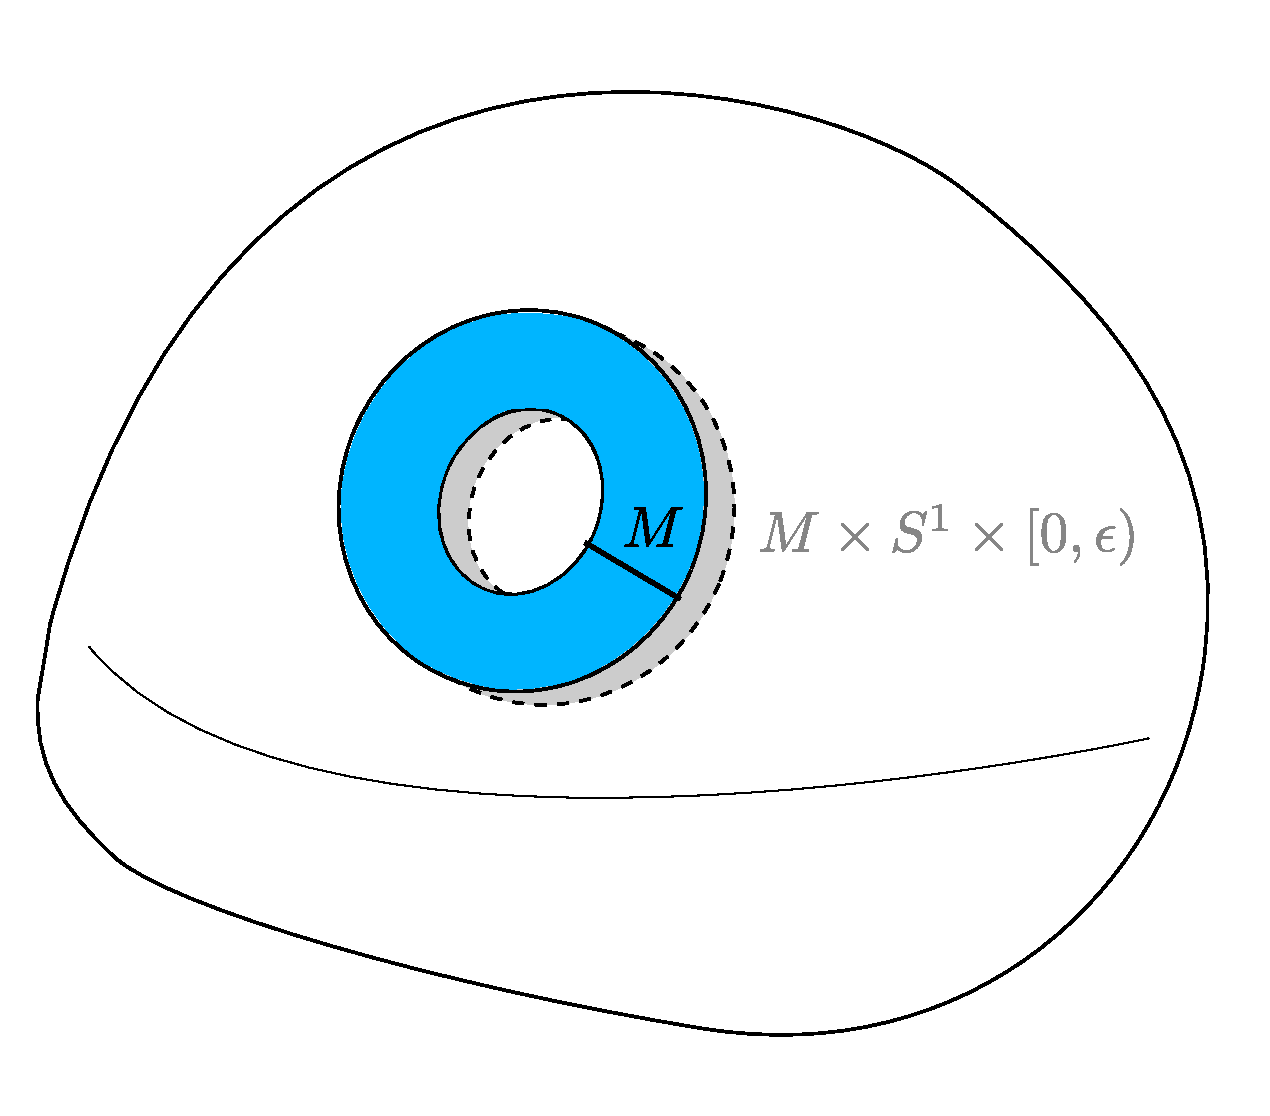
\includegraphics[width=\linewidth]{images/blow_down_before.pdf}
        \subcaption{The blue surface is a $\xi$-round boundary surface with (gray) neighborhood}
    \end{subfigure}\hspace*{.1\linewidth}
    \begin{subfigure}[t]{.6\linewidth}
        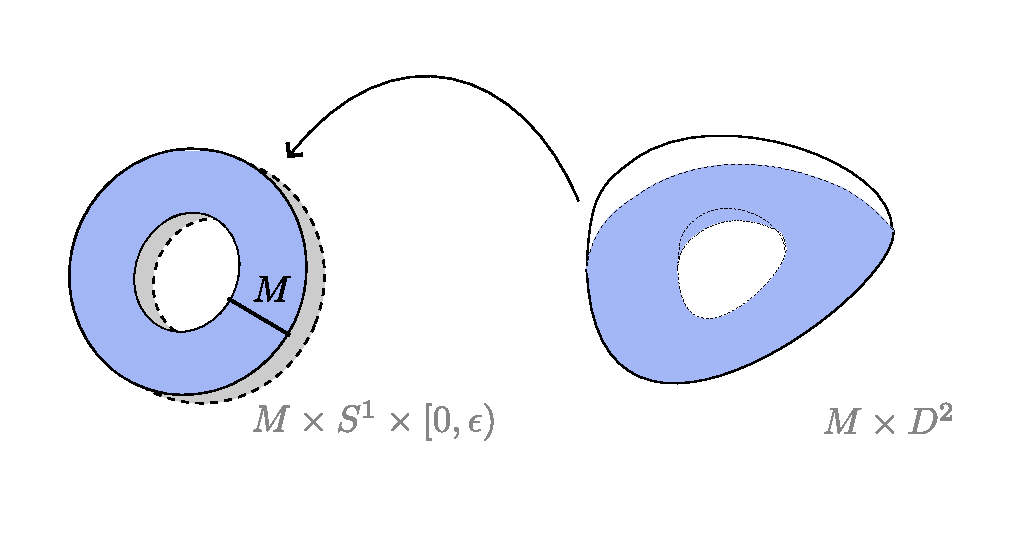
\includegraphics[width=\linewidth]{images/blow_down_topology.pdf}
        \subcaption{Topologically, the blowdown corresponds to gluing $M\times D^2$ 
        on top of the blue surface.}
    \end{subfigure}
    \begin{subfigure}{.9\linewidth}
        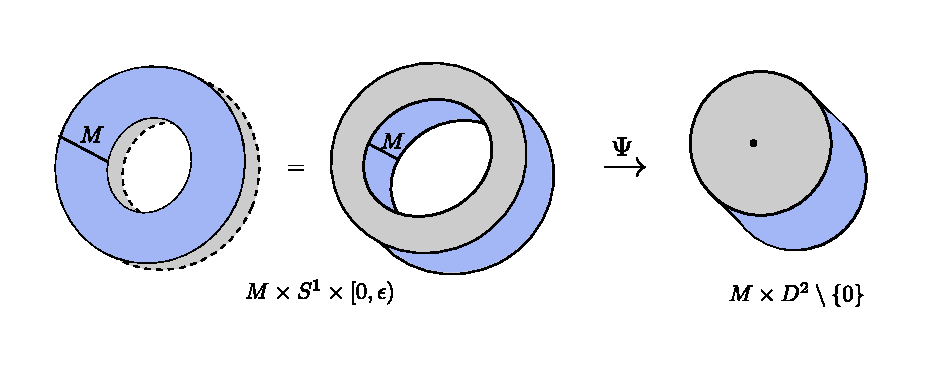
\includegraphics[width=\linewidth]{images/blow_down_contact.pdf}
        \subcaption{Visualization of $\Psi$: The neighborhood of the blue area
        $M \times S^1 \times \{0\}$ on the left is given by $M \times$ the gray annulus.
        In the middle, twist it so that the blue area sits on the inside.
        Applying $\Psi$ is simply retracting the inner circle of the gray annulus to a point.
        The blowdown effectively reduces the inner blue surface $M \times S^1$ to $M = M \times \{0\} \subset M \times D^2$.}
    \end{subfigure}
\end{figure}

Boundary components of Giroux domains are 
$\xi$-round hypersurfaces (\cite[Section 5.3]{MNW13}),
Therefore, after removal of a Giroux domain,
its boundary components can be blown down
These two steps together form the clean cut-out.
\section{A capping cobordism}
The following sections closely follow \cite[Section 6]{BGM22}.
\begin{comment}
In \cite[Section 6]{MNW13}, where the clean cut-out is first introduced,
it is shown that it corresponds to a symplectic cobordism.
The setting there is actually more general: The authors consider a Giroux
domain where already some of the boundary components have been blown down.
In this case, the situation is simpler: The Giroux domain 
$V_- \times S^1 \subset \operatorname{BO}(\Sigma, \dots)$
is directly obtained from the corresponding ideal Liouville domain $V_-$ by 
round contactization.
Its boundary is given by 
\[
    \partial V_- \times S^1 = \Gamma \times S^1.
\]
We want a cobordism from $\operatorname{BO}(\Sigma, \dots)$ to
the same manifold after clean cut-out of $V_- \times S^1$.
Topologically, the cobordism
\[
    W \coloneqq [0,1] \times \operatorname{BO}(\Sigma, \dots) \bigcup_{\{1\} \times \left(V_- \times S^1\right)} V_- \times D^2.
\]
fulfills the requirements: One boundary is simply 
$\operatorname{BO}(\Sigma, \dots)$.
The other boundary is 
\[
    \left[\operatorname{BO}(\Sigma, \dots) \setminus \left(V_- \times S^1\right)\right] 
    \cup_{\Gamma \times S^1} \Gamma \times D^2,
\]
which is homeomorphic to 
$\operatorname{BO}(\Sigma, \dots) \setminus \left(V_- \times S^1\right)$
with blown down boundary, which is exactly the desired clean cut-out.

Next, compute the contact structure on $\operatorname{BO}(\Sigma, \dots) \setminus \left(V_- \times S^1\right)$
with blown down boundary $\partial V_- \times S^1 = \Gamma \times S^1$.

This should be the contact boundary of $V_+ \times D^2$.
Topologically, that makes sense,
\[
    \partial (V_+ \times D^2) = V_+ \times S^1 \cup \partial V_+ \times D^2 = V_+ \times S^1 \cup_{\Gamma \times S^1} \Gamma \times D^2.
\]
However, it is unclear to me why $V_+ \times D^2$ should carry a \underline{symplectic structure}.

It should also be supported by the open book $\operatorname{OB}(V_+, \operatorname{id})$,
which, again, topologically, makes perfect sense, but I don't understand the
\underline{contact side of things}.
\end{comment}

For now, consider the easier case where no additional surgery is carried out on the Bourgeois manifold.
That makes the proof for the homological obstruction theorem easier to understand.
It can be generalized to the case with surgery later.
The idea is to cap off both sides (i.e. $V_+$ and $V_-$) of the convex decomposition
using the surgery procedure introduced in the last section.
Topologically, this will result in $\Gamma \times S^2$ and 
it will turn out to carry a stable Hamiltonian structure.

In \cite[Section 6]{MNW13}, where the clean cut-out is first introduced,
it is shown that it corresponds to a symplectic cobordism.
The setting there is actually more general: The authors consider a Giroux
domain where already some of the boundary components have been blown down.
In this case, the situation is simpler: The Giroux domain 
$V_\pm \times S^1 \subset \operatorname{BO}(\Sigma, \dots)$
is directly obtained from the corresponding ideal Liouville domain $V_\pm$ by 
round contactization.
Its boundary is given by 
\[
    \partial V_\pm \times S^1 = \Gamma \times S^1.
\]

Now, considering the manifold $(V_+ \cup_\Gamma V_-)\times S^1$, perform a clean cut-out
on both ends, i.e. remove the interior of $V_\pm \times S^1$ and blow down the boundary $\Gamma \times S^1$.
In order to do this properly, it is necessary to consider a neighborhood 
$\Gamma \times (-\delta, \delta)$ around the dividing set and 
instead of $V_\pm$ take $V_\pm' \coloneqq V_\pm \setminus \Gamma \times [0, \pm \delta]$.
Topologically, blowing down $\Gamma \times S^1$ yields $\Gamma \times D^2$.
As this is done on both sides, the result is 
\[
    \Gamma \times D^2 \cup_{\Gamma \times S^1 \times -\delta} \Gamma \times (-\delta,\delta) 
    \cup_{\Gamma \times S^1 \times +\delta} \Gamma \times D^2 \cong \Gamma \times S^2.
\]
For an example, see \cref{fig:cap_cobordism}.

\begin{figure}[h!]
    \begin{subfigure}[t]{.6\linewidth}
        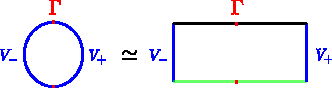
\includegraphics[trim=-.5cm -.5cm -.5cm -.5cm, width=\linewidth]{images/convex_decomposition_of_s1.pdf}
        \subcaption{The convex decomposition of $V = S^1$ 
        where the dividing set $\Gamma$ consists of two points is homotopic to a rectangle.}
    \end{subfigure}\hspace*{.1\linewidth}
    \begin{subfigure}[t]{.3\linewidth}
        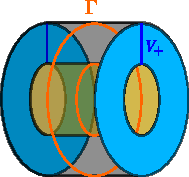
\includegraphics[trim=-.5cm -.5cm -.5cm -.5cm, width=\linewidth]{images/v_times_s1.pdf}
        \subcaption{Taking the product with $S^1$ yields this torus. This is now $V \times S^1$.}
    \end{subfigure}
    \begin{subfigure}{.9\linewidth}
        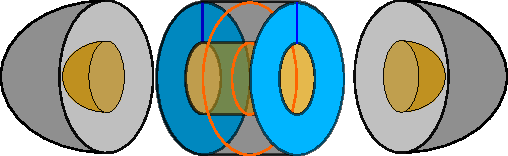
\includegraphics[trim=-.5cm -.5cm -.5cm -.5cm, width=\linewidth]{images/v_times_s1_with_caps.pdf}
        \subcaption{On the upper boundary of the capping cobordism, one adds $V_\pm \times D^2$-caps to the torus.}
    \end{subfigure}
    \begin{subfigure}{.9\linewidth}
        \centering
        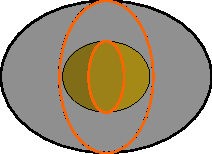
\includegraphics[trim=-.5cm -.5cm -.5cm -.5cm, width=.5\linewidth]{images/gamma_times_s2.pdf}
        \subcaption{As a result, the upper boundary of the cobordism is $\Gamma \times S^2$. In this case that amounts to an outer (gray) and an inner (green) sphere.}
    \end{subfigure}
    \caption[short]{The upper boundary of the capping cobordism.}
    \label{fig:cap_cobordism}
\end{figure}

This whole surgery procedure can be realized as applying a certain symplectic cobordism.
This is made precise in the following
\begin{lemma}(follows from \cite[Theorem 6.1]{MNW13}, cf. \cite[Lemma 6.1]{BGM22})\label{lem:capping_cobordism}
    There is a symplectic cobordism $(W, \omega)$ with negative (i.e. concave) 
    contact boundary $\partial_-W = V \times S^1$ and weakly convex positive boundary
    $\partial_+ W = \Gamma \times S^2$ where $\Gamma = \partial V$. 
    Moreover, there is a tubular neighborhood $(-\delta, 0] \times \partial_+ W$
    such that $\omega$ is of the form $d(e^t \alpha_\Gamma) + \omega_S$, 
    where $t \in (-\delta, 0]$ and 
    \begin{itemize}
        \item $\omega_S$ is an area form on $S^2$,
        \item $\alpha_\Gamma$ is a contact form on $\Gamma$.
    \end{itemize}
    Lastly, there are symplectic submanifolds $W_\pm$ , diffeomorphic to $V_\pm$, 
    such that $W\setminus W_\pm$ deformation retracts onto its negative boundary, 
    and such that $W_\pm$ intersect transversely, positively and in exactly one point, 
    each symplectic sphere in the previously described neighborhood 
    of the positive boundary $\partial_+ W$.
\end{lemma}

The submanifolds $W_\pm$ are basically $V_\pm \times 0 \subset V_\pm \times D^2$, i.e. 
the co-cores of the attached handles.
If these submanifolds are taken out, the effect of the capping is topologically trivial.
Therefore, the remaning cobordism is topologically just $\partial_- W\times [0,1]$.
This clearly deformation retracts to the negative boundary.
One can also construct a slightly modified deformation retract where instead 
of removing the co-cores, we remove slight push-offs 
(i.e. submanifolds that are obtained by shifting $W_\pm$ aside by a section of its normal bundle).
Then, $W_\pm$ retracts to $V_\pm$.
\section{Holomorphic spheres}
\begin{definition}
    Let $(\Sigma, j)$ be a Riemann surface and $(M, J)$ an almost-complex manifold. Then a smooth map
    \[
        u \colon \Sigma \to M
    \]
    is called $J$-holomorphic (or pseudoholomorphic) if its differential at every point is complex-linear, i.e.
    \[
        Tu \circ j = J \circ Tu.
    \]
\end{definition}

Pseudoholomorphic curves are used because holomorphic curves (where $M$ has to be a complex manifold) are to specific: 
A lot of manifolds don't even have a complex structure, whereas all symplectic manifolds admit an almost-complex structure.

%section 2.2.: Tameness and compatibility of almost complex structures on symplectic manifolds. Non-emptiness and contractibility of the total space
%
%4: We investigate the moduli space of holomorphic curves. The point is that parametrization shouldn't matter to a holomorphic curve.
%Therefore, one takes the space of all curves modulo reparametrization diffeos.
%Then, one tries to understand the resulting spaces. They are in some sense finite-dimensional (if Fredholm-regularity holds).
%This can be ensured in various ways. The goal, however, is always to understand the structure of these moduli spaces


\begin{definition}
    Let $(\Sigma, j)$ be a Riemann surface and $(M, J)$ an almost-complex manifold. Then a smooth map
    \[
        u \colon \Sigma \to M
    \]
    is called $J$-holomorphic (or pseudoholomorphic) if its differential at every point is complex-linear, i.e.
    \[
        Tu \circ j = J \circ Tu.
    \]
\end{definition}

Pseudoholomorphic curves are used because holomorphic curves (where $M$ has to be a complex manifold) are to specific: 
A lot of manifolds don't even have a complex structure, whereas all symplectic manifolds admit an almost-complex structure.

%section 2.2.: Tameness and compatibility of almost complex structures on symplectic manifolds. Non-emptiness and contractibility of the total space
%
%4: We investigate the moduli space of holomorphic curves. The point is that parametrization shouldn't matter to a holomorphic curve.
%Therefore, one takes the space of all curves modulo reparametrization diffeos.
%Then, one tries to understand the resulting spaces. They are in some sense finite-dimensional (if Fredholm-regularity holds).
%This can be ensured in various ways. The goal, however, is always to understand the structure of these moduli spaces

Last section, a cobordism from $M\times T^2$ to $\Gamma \times S^2$ was constructed.
Stacked on top of a hypothetical filling $W_\text{Bourgeois}$ of $M\times T^2$, this is a symplectic filling $W$ of $\Gamma \times S^2$.
$W$, like any symplectic manifold, admits a compatible almost complex structure $J$.
Now, the maps
\begin{align*}
    u_{(t,q)} \colon S^2 &\to W,\\
    y &\mapsto (t, q, y) \in (-\delta, 0] \times \underbrace{\Gamma \times S^2}_{= \partial_+ C}.
\end{align*}
are $J$-holomorphic curves.
%Why are they holomorphic?

Consider the connected component $\mathcal{M}$ of the moduli space of $J$-holomorphic spheres containing these $u_{t,q}$
and denote with $\mathcal{M}_*$ the corresponding marked moduli space with evaluation map
\[
    \operatorname{ev}\colon \mathcal{M}_* \to W.
\]
Define the respective Gromov compactifications $\overline{\mathcal{M}}$ and $\overline{\mathcal{M}}_*$.
Gromov proved that any sequence of holomorphic curves with finite energy bound converges to a
holomorphic curve that possibly has nodes or bubbles.
For now, just think of the Gromov compactification as adding all such limits of sequences to the space.
The finite energy bound follows from the fact that the homology class of the curve doesn't change.
\[
    E(u_k) = \int_{S^2} u_k^*(\omega) = \langle [u_k], [\omega] \rangle = \langle [S^2], [\omega]\rangle = \operatorname{const}.
\]
%What is a Gromov compactification precisely?

The following lemma describes the compactified moduli space close to the boundary.
\begin{lemma}(\cite[Lemma 6.3]{BGM22}, cf. \cite[page 334]{MNW13})\label{lem:local_uniqueness}
    Any curve in $\overline{\mathcal M}_*$ that intersects a small enough collar neighborhood
    \[
        (-\epsilon, 0] \times \Gamma \times S^2
    \]
    is already a reparametrization of a sphere $u_{t,q}$ (i.e. equivalent in the moduli space).
\end{lemma}

Now consider the evaluation map $\operatorname{ev}\colon \overline{\mathcal M}_* \to W$ close to the boundary (in the neighborhood of \cref{lem:local_uniqueness}).
There, the map is a diffeomorphism: Take any point $p  = (t, q, y) \in (-\epsilon, 0] \times \Gamma \times S^2$. 
Then, by construction there exists at least one holomorphic sphere ($u_{t,q}$) that intersects this point
and even has this point as marked point.
By \cref{lem:local_uniqueness}, any such curve is equivalent (as an element of the moduli space $\overline{\mathcal M}_*$) to $u_{t,q}$, hence the map is bijective.
The proof of smoothness is omitted here.

According to \cref{lem:capping_cobordism}, any such curve intersects $C_\pm$ transversely, positively and in exactly one point.
This gives rise to an intersection map
\[
    \mathcal{I}^\pm\colon \overline{\mathcal{M}} \to C_\pm.
\]

As $\partial C_\pm \subset \partial C$, a collar neighborhood of $\partial C_\pm$ is contained in a collar neighborhood of $\partial C$.
Therefore, the uniqueness lemma applies and it turns out that this map is a diffeomorphism close to the boundary $\partial \overline{\mathcal M}$.
We skip the smoothness and show that it is bijective.
\begin{itemize}
    \item Surjectivity: For $x \in C_\pm \cap (-\epsilon, 0] \times \Gamma \times S^2$, consider the coordinate representation $x = (t, q, y)$.
    Clearly, a preimage is given by $u_{t,q} \in \overline{\mathcal M}_*$ with marked point $x$. 
    \item Injectivity: The preimage is unique due to the uniqueness lemma.
\end{itemize}
\section{Proof sketch of the homological obstruction theorem}\label{sec:proof_hom_obstr}
The current situation is that 
\[
    M\times T^2 = V_- \times S_1 \bigcup_\Gamma V_+\times S_1
\] 
has a cobordism to $\Gamma \times S^2$.
The surgeries that turn $M\times T^2$ into $S^{2n+1}$ can be made disjoint from the dividing set, so it makes sense to talk about $\Gamma \subset S^{2n+1}$.
The full homology obstruction theorem states that any homology class in the dividing set $\Gamma$ that dies in a filling $W_\text{surg}$ of $S^{2n+1}$,
will also die in $V_\pm$.

For simplicity, in this thesis only a partial homology obstruction theorem will be proved, starting from a filling $W_\text{Bourgeois}$
of the Bourgeois manifold $M\times T^2$. What will be proved is that any homology class in the dividing set $\Gamma$ that dies in
$W_\text{Bourgeois}$ (all the more in $W$), will also die in $V_\pm$.

In order to make this more precise, define the inclusion maps
$i'\colon \Gamma \to \Gamma \times \{\operatorname{pt}\} \subset \Gamma \times S^2$ where $\operatorname{pt}$ is a point on the equator of $S^2$
and $i$ as the composition of $i'$ with the inclusion $\Gamma \times S^2 = \partial_+ C \hookrightarrow \partial W \hookrightarrow W$. 

Start with a cycle $z \in H_*(\Gamma, \mathbb Q)$ with $i_*(z) = 0 \in H_*(W, \mathbb{Q})$.
Consequently, there is a homology class $\sigma \in H_*(W, \mathbb Q)$ with boundary $i_*(z) = \partial \sigma$.
Any homology class in $\Gamma$ that dies in $W$ can be described in this way.
Intuitively, $\sigma$ can be pushed into $C_\pm$ in order to kill $z$ in $H_*(C_\pm, \mathbb{Q}) = H_*(V_\pm, \mathbb{Q})$.

More precisely, consider the commutative diagram
\[
\begin{tikzcd}
    \Gamma \arrow[r, hook, "i'"] \arrow[rrrr, bend left, "i"] \arrow[rrrdd, hook, "f_\pm"]
        & \Gamma \times S^2  = \partial W  \arrow[r, "\operatorname{ev}_\partial^{-1}", "\sim" below]
        & \partial \overline{\mathcal M}_* \arrow[r, hook, "j"]
        & \overline{\mathcal M}_*          \arrow[r, "\operatorname{ev}"] \arrow[d, twoheadrightarrow, "\pi"] \arrow[dd, bend right, "\mathcal I_\pi^\pm" left]
        & W \\
    &&& \overline{\mathcal M} \arrow[d, "\mathcal{I}^\pm"]  &   \\
    &&& C_\pm \simeq V_\pm                                  &   
\end{tikzcd}
\]
where $j$ and $\pi$ are the obvious inclusion respectively forgetful maps.
Recall that $\operatorname{ev}_\partial$ is the evaluation map restricted to the boundary of the moduli space. 
As proved in the last section, this map is a diffeomorphism close to the boundary and in particular on the boundary.
$\mathcal{I}^\pm\colon \overline{\mathcal{M}} \to W_\pm$ is the intersection map defined in the last section.
Finally, choose $\mathcal I_\pi^\pm$ and $f_\pm$ such that the diagram commutes.

The obstruction theorem states that already $f_{\pm,*}(z) = 0 \in H_*(C_\pm = V_\pm, \mathbb{Q})$.

Consider the set preimage $\operatorname{ev}^{-1}(\sigma) \subset \overline{\mathcal M}_*$.
As the boundary $\partial \sigma$ is contained in $\partial W$, the evaluation map is a diffeomorphism
and a neighborhood of $\partial \sigma$ is preserved under taking the preimage.
Away from this neighborhood, a slight perturbation might be necessary to make the resulting set a cycle in $\overline{\mathcal M}_*$.
%How does this work?
Clearly, the resulting cycle $\tau$ has boundary $\partial \tau \cong b$ and $\partial \tau$ is contained in the boundary $\partial \overline{\mathcal M}_*$.

%As $\pi$ maps $\partial \overline{\mathcal M}_*$ to $\partial \overline{\mathcal M}$, $\pi_*(\partial \tau)$ is contained in $\partial \overline{\mathcal M}$.
The following equation holds:
\begin{align*}
    \partial I_{\pi,*}^\pm(\tau) &= I_{\pi,*}^\pm(\partial \tau)\\
    &= I_{\pi, *}^\pm(\operatorname{ev}_{\partial, *}^{-1}(\partial \sigma))\\
    &= I_{\pi, *}^\pm(\operatorname{ev}_\partial^{-1}(i_*(z)))\\
    &= I_{\pi, *}^\pm\left((j \circ \operatorname{ev}_\partial^{-1} \circ i')_*(z)\right)\\
    &= f^\pm(z)
\end{align*}

As a result, $\left[f^\pm(z)\right] = \left[\partial I_{\pi,*}^\pm(\tau)\right] = 0 \in H_*(C_\pm, \mathbb Q) = H_*(V_\pm, \mathbb Q)$.
For a sketch of the proof, see \cref{fig:obstruction_proof_sketch}.

\begin{figure}
    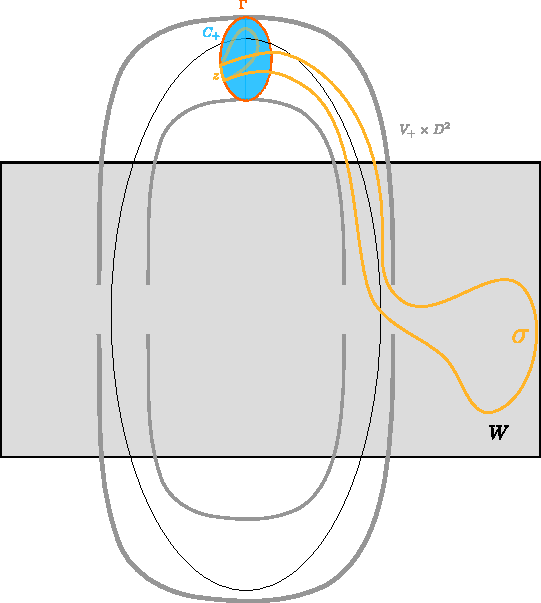
\includegraphics{images/obstruction_proof_sketch.pdf}
    \caption{Sketch of $W$ with the two handles. The homology class $\sigma \in H_*(W)$ with boundary $z \in H_*(\Gamma)$ is pushed to $H_*(C_\pm)$.}
    \label{fig:obstruction_proof_sketch}
\end{figure}
\section{Existence of the required homology class}\label{sec:homology_class}
The obstruction theorem says that any homology class in the dividing set that dies in the filling $W$, will also
die in $V_{\pm}$.
The goal is to prove that there is a nontrivial homology class $\beta \subset V_\pm$ that
comes from $\Gamma$, but dies in $W$. This contradicts the obstruction theorem and shows that there can be no filling.

\begin{lemma}
    There exists a homology class in $\Gamma$ that survives in $V_\pm$.
\end{lemma}
\begin{proof}
    By construction,
    \[
        V_\pm = \Sigma \times D^*S^1
    \]
    and
    \[
        \Gamma = \partial V_\pm = \partial \Sigma \times D^*S^1 \cup \textcolor{blue}{\Sigma} \times \left(\textcolor{blue}{S^1} \sqcup S^1\right).
    \]
    First construct a homology class in $\Sigma \times S^1$.
    The Künneth-formula for coefficient ring $\mathbb Z$ shows that
    \begin{multline}
        0 \to \bigoplus_{i+j = n} H_i(\Sigma) \otimes_{\mathbb Z} H_j(S^1) \to  H_n(\Sigma \times S^1)\\
        \to \bigoplus_{i+j = n-1} \operatorname{Tor}^\mathbb{Z}_1\left(H_i(\Sigma), H_j(S^1)\right) \to 0
    \end{multline}
    is an exact split sequence.
    Consequently,
    \[
        H_n(V_\pm) \cong \bigoplus_{i+j = n} H_i(\Sigma) \otimes_{\mathbb Z} H_j(S^1) \oplus 
        \bigoplus_{i+j = n-1} \operatorname{Tor}^\mathbb{Z}_1\left(H_i(\Sigma), H_j(S^1)\right).
    \]
    In \cref{sec:milnor}, homotopy and homology properties of $\Sigma$ (the Milnor fiber) were described.
    In particular, $H_{n-1}(\Sigma^{2n-2}) \neq 0$, as this is precisely half the dimension of the page.
    Together with $H_1(S^1) \neq 0$, this proves that the term $H_{n-1}(\Sigma) \otimes_{\mathbb Z} H_1(S^1)$ is nonzero. As a result, 
    there is a nonzero homology class in $H_n(\Sigma \times S^1) \hookrightarrow H_n(\Gamma)$.
    Inlusion into $V_\pm$ doesn't kill this homology group, as $S^1 \hookrightarrow D^*S^1$ is a homotopy equivalence,
    i.e. induces an isomorphism on homology level. 
    This proves the existence of a nontrivial homology class in $\Gamma$ that survives in $V_\pm$.
\end{proof}

Now, in the surgery case, with several modifications the inclusion
$V_+ \to W$ factors via $V_+ \hookrightarrow \partial W = S^{2n+1} \hookrightarrow W$.
On homology level, one gets
$H_n(V_+) \hookrightarrow H_n(S^{2n+1}) \hookrightarrow H_n(W)$.
As the middle term is $0$, any homology class coming from $V_+$ dies in the filling $W$.
This is the desired contradiction.
\newpage
\bibliographystyle{alpha}
\bibliography{bibliography}
\end{document}